\documentclass[12pt]{article}

\usepackage[margin=0.8 in]{geometry}
\usepackage{amsmath}
\usepackage{amssymb}
\usepackage{mathtools}
\usepackage{enumerate}
\usepackage{verbatim}
\usepackage{amsthm}
\usepackage{hyperref}

\title{}
%\content{}



\let \proj \undefined
\newcommand{\p}{\partial}
\newcommand{\R}{ \mathbb{R}}

\DeclareMathOperator{\proj}{proj}
\newcommand{\sS}{\mathscr{S}}
\DeclareMathOperator{\comp}{comp}
\newcommand{\A}{\mathcal{A}}
\newcommand{\D}{\mathcal{D}}
\newcommand{\e}{\epsilon}
\newcommand{\et}{\tilde{\e}}
\newcommand{\vr}{\vec{r}{}}
\newcommand{\vF}{\vec{F}}
\newcommand{\triple}{\iiint_E f(x,y,z)dV}
\renewcommand{\lg}{\langle}
\newcommand{\rg}{\rangle}
\newcommand{\Q}{\frac{\p Q}{\p x}}
\renewcommand{\P}{\frac{\p P}{\p y}}
\let\implies\Rightarrow
\newcommand{\n}{\nabla}
\newcommand{\Fline}{\vF\cdot d\vr}
\newcommand{\vi}{\vec{i}}
\newcommand{\vj}{\vec{j}}
\newcommand{\vk}{\vec{k}}
\DeclareMathOperator{\curl}{curl}
\newcommand{\vn}{\vec{n}}
\newcommand{\vS}{\vec{S}}
\newcommand{\flux}{\iint_S \vF\cdot d\vS}

\newcommand{\rcross}{\vr_u\times\vr_v} 

\let\sq \sqrt


\newenvironment{solution}
  {\begin{proof}[Solution]}
  {\end{proof}
  
  }
\newtheorem{example}{Example}
\newtheorem{exercise}{Exercise}
\newtheorem{theorem}{Theorem}
\newtheorem{cor}{Corollary}
\newtheorem{defn}{Definition}


\begin{document}



\section*{Surface Integrals}

What to know:
\begin{enumerate}
\item Be able to set up and compute surface integrals of scalar functions.
\item Know that surface integrals of scalar function don't depend on the orientation of the surface.
\item Be able to set up an compute surface integrals of vector fields, being careful about orientations.
\end{enumerate}





In this section we'll make sense of integrals over surfaces. In a sense, the content of this section is very analogous to the one discussing line integrals, except here we'll be working with two dimensional objects instead of one dimensional.

Recall that when we talked about line integrals, some of them depended on the parameterization of the curve, and more specifically on the direction the curve was transversed, whereas others didn't. It's therefore natural to expect that we might have to deal with some similar behavior when discussing surface integrals, except in this two dimensional setting we are going to use the concept of orientation discussed in the previous section.

\subsection*{Surface integrals of scalar functions}
You might remember that when we discussed line integrals, the main motivation for them was the fact that we wanted to use them in order to compute the area of a fence or curtain above a curve on the plane, but we also said that they can be used to calculate the mass of a wire: If a wire lies on the curve $c(t)$ in $\R^3$ and its density at the point $(x,y,z)$ is $\rho(x,y,z)$ then its mass is given by $$m=\int_c \rho(x,y,z)ds.$$


Now we will define integrals on surfaces, so that we can compute the mass of a piece of aluminum foil with non constant density function folded in $\R^3$.


\begin{figure}[h]
\begin{center}
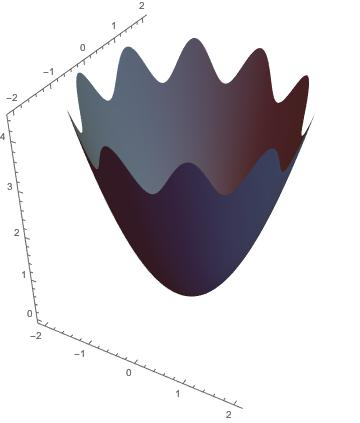
\includegraphics[scale=.3]{foil.jpeg}
\caption{A nicely folded piece of aluminum foil}
\end{center}
\end{figure}

\begin{defn}
Suppose $S$ is a parametric surface in $\R^3$ with parametrization $\vr(u,v)$, $(u,v)\in D$ and $f(x,y,z)$ is a continuous function on $S$. Then we define the \textbf{surface integral of $f$ over $S$} to be $$\iint_S f(x,y,z)dS:=\iint_D f(\vr(u,v))|\rcross(u,v)| dA.$$
\end{defn}

\textbf{Remarks:}
\begin{enumerate}
\item As you might remember from a couple of sections ago, we denoted $dS:=|\rcross|dA$, so the above notation makes sense.
\item The mass of a piece of aluminum foil lying on the surface $S$ with density function $\rho(x,y,z)$ is given by the formula $$m=\iint_S \rho(x,y,z)dS.$$ 
\end{enumerate}

\begin{example} Find the mass of a piece of aluminum foil occupying the surface $z=x^2+y^2$, $z\leq 4$, if it has density function $\rho(x,y,z)=\frac{z}{\sqrt{4z+1}}.$
\end{example}
\begin{solution}${}$\\
\noindent\textbf{1st Way:} We will parametrize the paraboloid $z=x^2+y^2$ as a surface of revolution, namely we let $$\vr(u,v)=\lg \sqrt{v}\cos(u),\sqrt{v}\sin(u),v\rg, (u,v)\in [0,2\pi]\times [0,4].$$

We find $$\vr_u=\lg -\sqrt{v}\sin(u),\sqrt{v}\cos(u),0\rg,$$
$$\vr_v=\lg \frac{1}{2\sqrt{2}}\cos(u),\frac{1}{2\sqrt{v}}\sin(u),1\rg$$
and therefore
$$\rcross(u,v)=\lg \sqrt{v}\cos(u),\sq{v}\sin(u),-\frac{1}{2}\rg.$$
Note that the $z$ coordinate is negative, so this corresponds to a \textbf{downward} orientation.

Then we find $$|\rcross(u,v)|=\sqrt{v+\frac{1}{4}}$$ and finally $$m=\int_0^2\pi\int_0^4 \frac{v}{\sq{4v+1}}\sq{v+\frac{1}{4}}dvdu=\dots=8\pi.$$

\vspace {.2 in}


\noindent\textbf{2nd Way:} We parametrize the paraboloid as a graph. We write $$\vr(u,v)=\lg u,v,u^2+v^2\rg, (u,v)\in D.$$

To find $D$, we intersect $z=x^2+y^2$, $z=4$ and find $$D=\{(u,v):u^2+v^2\leq 4\}.$$ 

Then, following a similar procedure, we find $\vr=\lg 1,0,2u\rg$, $\vr=\lg 0,1,2v\rg$ and $$\rcross=\lg -2u, -2v, 1\rg,$$ therefore $$|\rcross(u,v)|=\sq{4u^2+4v^2+1}.$$ Note that the orientation given by $\rcross$ now \textbf{upward}.

 Finally, we find $$m =\iint_D \frac{u^2+v^2}{\sq{4(u^2+v^2)+1}}\sq{4u^2+4v^2+1}dA=\dots=8\pi$$ 
using polar coordinates.
\end{solution}

Note that even we used two different parametrizations for which $\rcross$ gives different orientations, and still found the same result.

\vspace {.2 in}


We have the following:

\textbf{Surface integrals of scalar functions do not depend on the orientation.}

\vspace {.2 in}


Another useful formula for surface integrals of scalar functions\textbf{ when the surface is the graph of a function }$g(u,v),$ for $(u,v)\in D$ is $$\iint_S f dS=\iint_Df(u,v,g(u,v))\sq{\left( \frac{\p g }{\p u}\right )^2+\left( \frac{\p g}{\p v}\right )^2+1}dA$$



\subsection*{Surface integrals of vector fields}

A fairly intuitive motivation for defining surface integrals of vector fields is the situation when we'd like to understand how to find the mass of fluid passing through a fishing net, in a certain direction, in unit time.

\begin{figure}[h]
\begin{center}
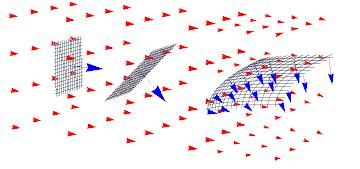
\includegraphics[scale=.6]{stream.jpeg}
\end{center}
\end{figure}

Let's look at a special case when we have a fishing net in the shape of a rectangle of area $A$ with unit normal vector $\vec{n}$ pointing towards our preferred direction, and suppose that our fluid has density $\rho$ and constant velocity $\vec{v}$ near the fishing net. If the fishing net were perpendicular to the water stream, like the one on the left, the mass of fluid per unit time would be $$m=\rho|\vec{v}|A,$$ but if it were not, like the one in the middle, we'd have to take into account that we only care about the component of the fluid stream that crosses the net orthogonally. We would do this by projecting the velocity vector field in the direction perpendicular to the net (the direction of the blue vector in the picture), that is, finding the dot product with $\vec{n}$, and we'd have $$m=\rho \vec{v}\cdot\vec{n} A.$$

What if the fishing net were occupying a more complicated surface, like the one on the right, and the velocity of the fluid weren't constant? A reasonable thing to do would be to break it into small pieces that look like rectangles, and where the velocity of the fluid is almost constant, work as before, and then sum those small masses we found. Making the rectangles smaller and smaller amounts to our procedure becoming an integration over the surface.

We end up defining:

\begin{defn}
Let $S$ be an oriented parametric surface with orientation determined by the unit normal vector field $\vn$ and $\vF$ be a continuous vector field. We define the \textbf{surface integral of $\vF$ over $S$} or \textbf{flux of $\vF$ across $S$} to be $$\iint_S\vF\cdot d \vS :=\iint_S \vF\cdot \vn dS.$$
\end{defn}

\textbf{Remark:} The right hand side is a surface integral of $\vF\cdot \vn$, which is a scalar function. We saw how to make sense of those in the first part of this section.
\vspace{.2 in}

Let's expand the definition and try to find an easier to use formula. Suppose $S$ is parametrized as $\vr(u,v) $ and recall that $\vn=\pm\dfrac{\rcross}{|\rcross|}$.

Then we have:
\begin{align*}
\iint_S\vF\cdot d \vS =&\iint_S \vF\cdot \vn dS\\
=& \iint_S \vF\cdot \left (\pm\dfrac{\rcross}{|\rcross|}\right )dS\\
=& \iint_D \vF\left (\vr(u,v)\right )\cdot \left (\pm\dfrac{\rcross}{|\rcross|}\right )|\rcross|dA\\
=& \pm\iint_D \vF\left (\vr(u,v)\right )\cdot (\rcross(u,v)) dA
\end{align*}
 
So, we have:

\begin{itemize}
\item If the orientation is such that $\vn=\dfrac{\rcross}{|\rcross|}$, then \begin{equation}\iint_S\vF\cdot d \vS=\iint_D \vF\left (\vr(u,v)\right )\cdot (\rcross(u,v)) dA \end{equation} whereas:

\item  if the orientation is such that $\vn=-\dfrac{\rcross}{|\rcross|}$, then \begin{equation}
 \label{eq1}\iint_S\vF\cdot d \vS=-\iint_D \vF\left (\vr(u,v)\right )\cdot (\rcross(u,v))dA .
 \end{equation}
\end{itemize}
Essentially, once we have a parametrization, the two formulas above save us from the trouble of finding $|\rcross|$.

\vspace{.2 in}

We can use the above to find an easier expression \textbf{in the case when $S$ is the graph of a function} $g(u,v)$, $(u,v)\in D$. As observed in Example 1 the previous section, when we use the parametrization $\vr(u,v)=\lg u,v,g(u,v)\rg$, then the vector field $\rcross(u,v)=\lg u,v,g(u,v)\rg=\lg -\dfrac{\p g}{\p u},-\dfrac{\p g}{\p v},1\rg$ corresponds to upward orienation. So, suppose that $\vF=\lg P,Q,R\rg$ and we find that
\begin{itemize}
\item If the orientation of $S$ is upward, then $$\iint_S \vF\cdot d\vS=\iint_D-\dfrac{\p g}{\p u}P-\dfrac{\p g}{\p v}Q+R dA$$

whereas

\item If the orientation of $S$ is downward, then $$\iint_S \vF\cdot d\vS=-\iint_D-\dfrac{\p g}{\p u}P-\dfrac{\p g}{\p v}Q+R dA$$
\end{itemize}

\begin{example}

Let $S$ be the upper hemisphere of the unit sphere oriented \textbf{downwards}, and let $\vF=\lg -y,x,1\rg.$ Compute the flux of $\curl\vF $ across $S$.
\end{example}
\begin{solution}
We compute $\curl \vF$ and find $$\curl\vF=\lg 0, 0 ,2\rg.$$ 

Then, we parametrize the upper half sphere as $$\vr(u,v)=\lg \sin(u)\cos(v),\sin(u)\sin(v),\cos(u)\rg,\text{ for }(u,v)\in[0,\frac{\pi}{2}]\times[0,2\pi].$$ We found in Example 2 of the previous section that $$\rcross(u,v)=\lg\sin^2(u)\cos(v),\sin^2(u)\sin(v),\cos(u)\sin(u)\rg$$ gives outward orientation in the case of the entire sphere, so it would give upward orientation in the case of the upper hemisphere. Therefore, we work with formula \eqref{eq1} and find \begin{align*}
\iint_S \curl\vF\cdot d\vS=&-\int_0^{2\pi}\int_0^{\frac{\pi}{2}}\lg 0, 0 ,2\rg\cdot \lg\sin^2(u)\cos(v),\sin^2(u)\sin(v),\cos(u)\sin(u)\rg du dv\\
=&-\int_0^{2\pi}\int_0^{\frac{\pi}{2}}2\cos(u)\sin(u)du dv\\
=&-2\pi,
\end{align*}
using the double angle formula $\sin(2t)=2\sin(t)\cos(t) $ or a $u$ substitution.
\end{solution}

\textbf{Remark:} The negative sign is expected in the answer: The vector field $\curl\vF=\lg 0,0,2\rg$ is pointing upwards, which is in direction ``opposite to the preferred one'', which is downward.


\end{document}

